\chapter{High-Concurrency Systems}

\section{Introduction}

Modern internet-scale systems must handle thousands to millions of concurrent users while maintaining low latency and high throughput. High-concurrency systems combine operating system principles, networking, distributed systems, and efficient software architecture.

Examples include:

\begin{itemize}
\item Web servers
\item API gateways
\item Database servers
\item Message brokers
\item Streaming platforms
\item Cloud services
\end{itemize}

Understanding high-concurrency systems is essential for SDE, Backend Engineering, Distributed Systems, and System Design interviews.

\section{What High Concurrency Means}

Concurrency refers to the ability of a system to manage multiple tasks simultaneously.

Examples:

\begin{itemize}
\item 10,000 simultaneous TCP connections
\item Millions of HTTP requests per minute
\item Thousands of database queries per second
\end{itemize}

High concurrency does not necessarily mean high parallelism.

\begin{itemize}
\item Concurrency = Managing many tasks
\item Parallelism = Executing many tasks simultaneously
\end{itemize}

\section{Concurrency Challenges}

Major challenges include:

\begin{itemize}
\item Resource contention
\item Synchronization overhead
\item Memory consumption
\item Context switching
\item Lock contention
\item Kernel bottlenecks
\item Queue buildup
\item Latency spikes
\end{itemize}

\section{Throughput vs Latency}

\subsection{Throughput}

Amount of work completed per unit time.

Examples:

\begin{itemize}
\item Requests per second (RPS)
\item Transactions per second (TPS)
\item Queries per second (QPS)
\end{itemize}

\subsection{Latency}

Time required to complete a request.

Examples:

\begin{itemize}
\item 10 ms API response
\item 2 ms database query
\end{itemize}

\begin{table}[H]
\centering
\begin{tabular}{lll}
\toprule
Metric & Meaning & Goal \\
\midrule
Throughput & Work Completed & High \\
Latency & Response Time & Low \\
\bottomrule
\end{tabular}
\caption{Throughput vs Latency}
\end{table}

\section{Thread-per-Request Model}

Traditional servers allocate one thread per request.

\begin{figure}[H]
\centering
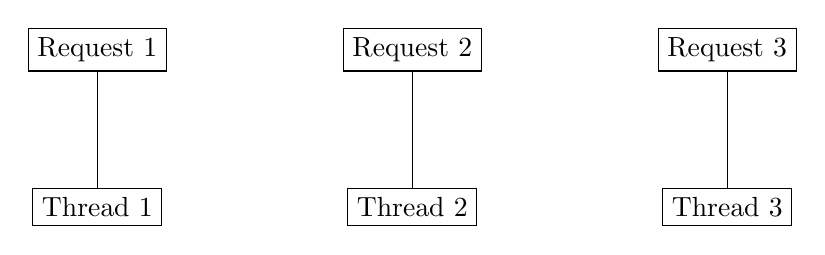
\begin{tikzpicture}
\node[draw] (req1) at (-4,2) {Request 1};
\node[draw] (req2) at (0,2) {Request 2};
\node[draw] (req3) at (4,2) {Request 3};

\node[draw] (t1) at (-4,0) {Thread 1};
\node[draw] (t2) at (0,0) {Thread 2};
\node[draw] (t3) at (4,0) {Thread 3};

\draw (req1)--(t1);
\draw (req2)--(t2);
\draw (req3)--(t3);
\end{tikzpicture}
\caption{Thread-per-Request Model}
\end{figure}

Advantages:

\begin{itemize}
\item Simple design
\item Easy programming model
\end{itemize}

Problems:

\begin{itemize}
\item High memory usage
\item Context switching overhead
\item Poor scalability
\end{itemize}

\section{Event-Driven Architecture}

Instead of dedicating one thread per request, an event loop handles many connections.

\begin{figure}[H]
\centering
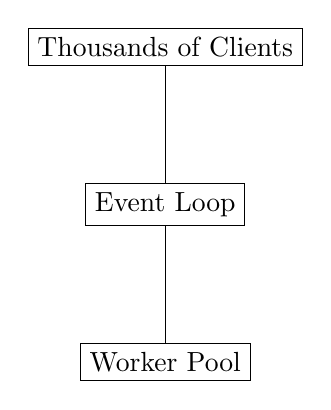
\begin{tikzpicture}
\node[draw] (clients) at (0,4) {Thousands of Clients};
\node[draw] (eventloop) at (0,2) {Event Loop};
\node[draw] (workers) at (0,0) {Worker Pool};

\draw (clients)--(eventloop);
\draw (eventloop)--(workers);
\end{tikzpicture}
\caption{Event-Driven Architecture}
\end{figure}

Benefits:

\begin{itemize}
\item Low memory usage
\item Better scalability
\item Efficient I/O handling
\end{itemize}

\section{Reactor Pattern}

The Reactor pattern waits for events and dispatches handlers.

Workflow:

\begin{enumerate}
\item Event arrives
\item Event loop detects readiness
\item Appropriate handler executes
\item Response generated
\end{enumerate}

Examples:

\begin{itemize}
\item Nginx
\item Redis
\item Node.js
\end{itemize}

\begin{figure}[H]
\centering
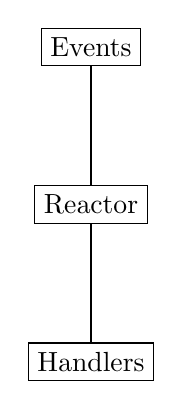
\begin{tikzpicture}
\node[draw] (events) at (0,4) {Events};
\node[draw] (reactor) at (0,2) {Reactor};
\node[draw] (handler) at (0,0) {Handlers};

\draw (events)--(reactor);
\draw (reactor)--(handler);
\end{tikzpicture}
\caption{Reactor Pattern}
\end{figure}

\section{Proactor Pattern}

The Proactor pattern uses asynchronous operations.

Workflow:

\begin{enumerate}
\item Submit asynchronous request
\item Kernel performs work
\item Completion event generated
\item Completion handler executes
\end{enumerate}

Examples:

\begin{itemize}
\item Windows IOCP
\item Linux io\_uring
\end{itemize}

\section{Non-Blocking I/O}

Non-blocking I/O returns immediately.

Example:

\begin{lstlisting}[style=interviewcode,language=C]
fcntl(fd, F_SETFL, O_NONBLOCK);
\end{lstlisting}

Benefits:

\begin{itemize}
\item Efficient event loops
\item Better scalability
\end{itemize}

\section{Asynchronous I/O}

Asynchronous I/O allows processing to continue while operations execute.

\begin{figure}[H]
\centering
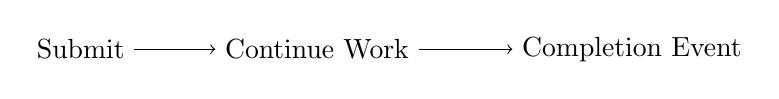
\begin{tikzpicture}
\node (submit) at (0,0) {Submit};
\node (continue) at (3,0) {Continue Work};
\node (complete) at (7,0) {Completion Event};

\draw[->] (submit)--(continue);
\draw[->] (continue)--(complete);
\end{tikzpicture}
\caption{Asynchronous I/O}
\end{figure}

Advantages:

\begin{itemize}
\item High concurrency
\item Reduced idle waiting
\end{itemize}

\section{Thread Pools}

Creating threads for every request is expensive.

Thread pools maintain reusable workers.

\begin{figure}[H]
\centering
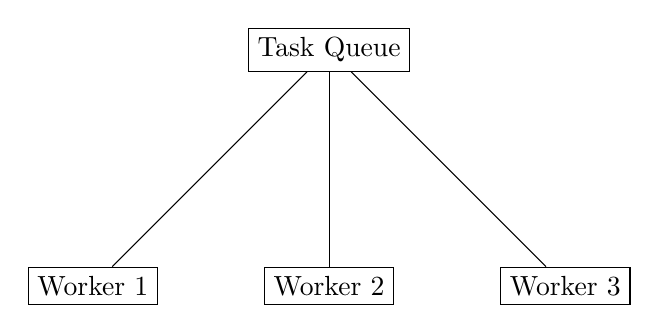
\begin{tikzpicture}
\node[draw] (queue) at (0,3) {Task Queue};

\node[draw] (w1) at (-3,0) {Worker 1};
\node[draw] (w2) at (0,0) {Worker 2};
\node[draw] (w3) at (3,0) {Worker 3};

\draw (queue)--(w1);
\draw (queue)--(w2);
\draw (queue)--(w3);
\end{tikzpicture}
\caption{Thread Pool}
\end{figure}

Benefits:

\begin{itemize}
\item Reduced creation overhead
\item Better throughput
\item Predictable resource usage
\end{itemize}

\section{Connection Pools}

Opening database connections is expensive.

Connection pools maintain reusable connections.

\begin{figure}[H]
\centering
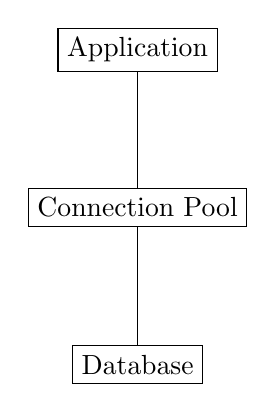
\begin{tikzpicture}
\node[draw] (app) at (0,4) {Application};

\node[draw] (pool) at (0,2) {Connection Pool};

\node[draw] (db) at (0,0) {Database};

\draw (app)--(pool);
\draw (pool)--(db);
\end{tikzpicture}
\caption{Connection Pool}
\end{figure}

Benefits:

\begin{itemize}
\item Reduced latency
\item Better scalability
\item Resource reuse
\end{itemize}

\section{Load Balancing}

Load balancers distribute traffic across servers.

Algorithms:

\begin{itemize}
\item Round Robin
\item Least Connections
\item Weighted Round Robin
\item Consistent Hashing
\end{itemize}

\begin{figure}[H]
\centering
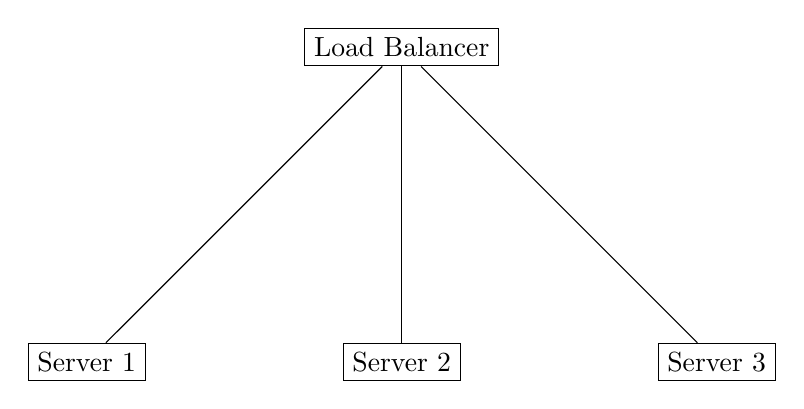
\begin{tikzpicture}
\node[draw] (lb) at (0,4) {Load Balancer};

\node[draw] (s1) at (-4,0) {Server 1};
\node[draw] (s2) at (0,0) {Server 2};
\node[draw] (s3) at (4,0) {Server 3};

\draw (lb)--(s1);
\draw (lb)--(s2);
\draw (lb)--(s3);
\end{tikzpicture}
\caption{Load Balancing}
\end{figure}

\section{Context Switching Costs}

Context switching requires:

\begin{itemize}
\item Register saving
\item Register restoration
\item Cache disruption
\item Scheduler overhead
\end{itemize}

Excessive threads lead to:

\begin{itemize}
\item Increased CPU overhead
\item Reduced throughput
\item Higher latency
\end{itemize}

\section{Kernel Bottlenecks}

Common bottlenecks include:

\begin{itemize}
\item Lock contention
\item Scheduler overhead
\item Interrupt handling
\item Socket management
\item File descriptor limits
\end{itemize}

\section{Resource Contention}

Multiple threads competing for resources can reduce performance.

Examples:

\begin{itemize}
\item CPU contention
\item Memory contention
\item Lock contention
\item Disk contention
\end{itemize}

Mitigation strategies:

\begin{itemize}
\item Lock-free structures
\item Sharding
\item Partitioning
\item Horizontal scaling
\end{itemize}

\section{Backpressure}

Backpressure prevents overload.

Example:

\begin{enumerate}
\item Producer generates faster than consumer
\item Queue grows
\item System slows producer
\end{enumerate}

Benefits:

\begin{itemize}
\item Stability
\item Controlled latency
\item Avoiding crashes
\end{itemize}

\section{Queue-Based Architectures}

Queues decouple producers and consumers.

Examples:

\begin{itemize}
\item Kafka
\item RabbitMQ
\item Amazon SQS
\end{itemize}

\begin{figure}[H]
\centering
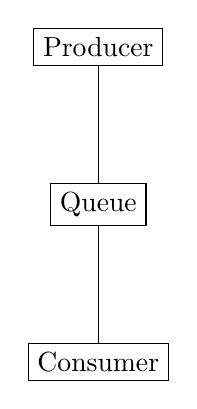
\begin{tikzpicture}
\node[draw] (producer) at (0,4) {Producer};
\node[draw] (queue) at (0,2) {Queue};
\node[draw] (consumer) at (0,0) {Consumer};

\draw (producer)--(queue);
\draw (queue)--(consumer);
\end{tikzpicture}
\caption{Queue-Based Architecture}
\end{figure}

\section{High-Concurrency Web Servers}

Modern web servers rely on:

\begin{itemize}
\item epoll
\item Event loops
\item Worker pools
\item Non-blocking sockets
\end{itemize}

Examples:

\begin{itemize}
\item Nginx
\item Envoy
\item HAProxy
\end{itemize}

\subsection{Nginx-Style Architecture}

\begin{figure}[H]
\centering
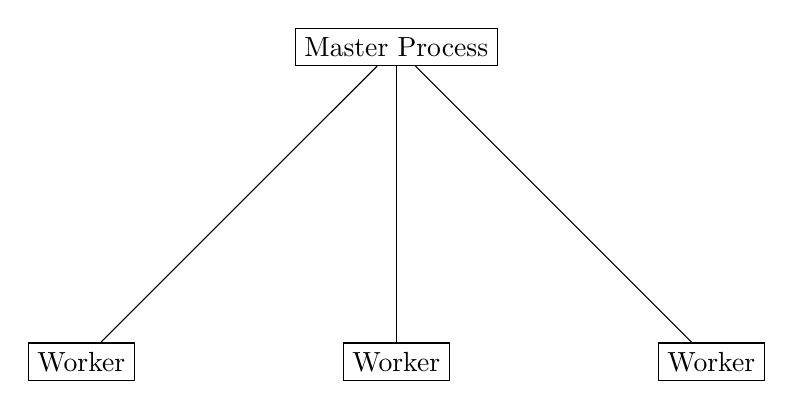
\begin{tikzpicture}
\node[draw] (master) at (0,4) {Master Process};

\node[draw] (w1) at (-4,0) {Worker};
\node[draw] (w2) at (0,0) {Worker};
\node[draw] (w3) at (4,0) {Worker};

\draw (master)--(w1);
\draw (master)--(w2);
\draw (master)--(w3);
\end{tikzpicture}
\caption{Nginx Worker Architecture}
\end{figure}

\section{High-Concurrency Databases}

Databases use:

\begin{itemize}
\item Connection pools
\item Buffer pools
\item Async replication
\item Lock management
\item Query optimization
\end{itemize}

Examples:

\begin{itemize}
\item PostgreSQL
\item MySQL
\item Cassandra
\item MongoDB
\end{itemize}

\section{Modern Backend Architectures}

Modern systems commonly combine:

\begin{itemize}
\item Load balancers
\item API gateways
\item Microservices
\item Message queues
\item Databases
\item Distributed caches
\end{itemize}

\begin{figure}[H]
\centering
\begin{tikzpicture}
\node[draw] (client) at (0,6) {Clients};

\node[draw] (lb) at (0,4) {Load Balancer};

\node[draw] (api) at (0,2) {API Services};

\node[draw] (mq) at (-3,0) {Queue};
\node[draw] (db) at (3,0) {Database};

\draw (client)--(lb);
\draw (lb)--(api);
\draw (api)--(mq);
\draw (api)--(db);
\end{tikzpicture}
\caption{Modern Backend Architecture}
\end{figure}

\section{Dedicated Interview Section: How a Web Server Handles Millions of Requests}

Modern web servers use:

\begin{enumerate}
\item Non-blocking sockets
\item epoll or kqueue
\item Event loops
\item Worker processes
\item Load balancing
\item Efficient memory management
\end{enumerate}

A single worker can manage thousands of connections because idle connections consume minimal CPU.

\section{Dedicated Interview Section: Why Thread-per-Request Does Not Scale}

Problems:

\begin{itemize}
\item Large memory consumption
\item High context switching overhead
\item Scheduler pressure
\item Lock contention
\end{itemize}

Example:

\begin{itemize}
\item 100,000 requests
\item 100,000 threads
\item Several hundred GB memory required
\end{itemize}

Event-driven architectures solve this issue.

\section{Dedicated Interview Section: Event-Driven Systems Explained}

Event-driven systems process events rather than blocking per request.

Workflow:

\begin{enumerate}
\item Event arrives
\item Event loop receives notification
\item Handler executes
\item Response returned
\end{enumerate}

Examples:

\begin{itemize}
\item Node.js
\item Nginx
\item Redis
\item Netty
\end{itemize}

Benefits:

\begin{itemize}
\item High scalability
\item Low resource consumption
\item Excellent concurrency
\end{itemize}

\section{Key Takeaways}

\begin{keytakeaways}
High-concurrency systems are designed to handle massive numbers of simultaneous requests while maintaining low latency and high throughput. Traditional thread-per-request architectures suffer from memory overhead and context-switching costs. Modern systems use event-driven architectures, non-blocking I/O, asynchronous processing, thread pools, connection pools, and load balancing. Reactor and Proactor patterns are common foundations for scalable servers. Backpressure, queue-based designs, and efficient resource management are critical for maintaining stability under heavy load.
\end{keytakeaways}

\section{Interview Questions with Answers}

\begin{enumerate}
\item What is high concurrency?\\
The ability to manage many simultaneous tasks or requests.

\item What is throughput?\\
Amount of work completed per unit time.

\item What is latency?\\
Time required to complete a request.

\item Why is latency important?\\
Users perceive system responsiveness through latency.

\item What is thread-per-request?\\
A model where each request receives a dedicated thread.

\item Why does thread-per-request not scale?\\
Memory and context-switching overhead.

\item What is an event-driven architecture?\\
Architecture based on processing events through handlers.

\item What is the Reactor pattern?\\
An event demultiplexer that dispatches handlers.

\item What is the Proactor pattern?\\
Completion-based asynchronous processing.

\item What is non-blocking I/O?\\
I/O that returns immediately.

\item What is asynchronous I/O?\\
I/O that completes in the background.

\item Why are thread pools useful?\\
They reduce thread creation overhead.

\item What is a connection pool?\\
A reusable set of database connections.

\item Why use connection pools?\\
Reduce connection setup costs.

\item What is load balancing?\\
Traffic distribution across servers.

\item What causes context-switch overhead?\\
Saving and restoring execution state.

\item What is lock contention?\\
Threads competing for locks.

\item What is backpressure?\\
Mechanism preventing overload.

\item Why use message queues?\\
Decouple producers and consumers.

\item What is epoll?\\
Linux event notification mechanism.

\item Why is epoll scalable?\\
Reports only ready descriptors.

\item How does Nginx scale?\\
Workers + epoll + event loops.

\item What is a worker process?\\
A process handling client requests.

\item Why are event loops efficient?\\
Minimal threads handle many connections.

\item What architecture powers most modern backend systems?\\
Event-driven, distributed architectures.
\end{enumerate}

\section{MCQs with Answers}

\begin{enumerate}

\item Throughput measures:
\begin{enumerate}[label=(\alph*)]
\item Delay
\item Work Completed
\item Memory
\item CPU
\end{enumerate}
Answer: (b)

\item Latency measures:
\begin{enumerate}[label=(\alph*)]
\item Response Time
\item CPU Usage
\item Memory
\item Storage
\end{enumerate}
Answer: (a)

\item Thread-per-request allocates:
\begin{enumerate}[label=(\alph*)]
\item One Process
\item One Queue
\item One Thread
\item One CPU
\end{enumerate}
Answer: (c)

\item Nginx primarily uses:
\begin{enumerate}[label=(\alph*)]
\item Reactor Pattern
\item FCFS
\item Paging
\item Segmentation
\end{enumerate}
Answer: (a)

\item Proactor relies on:
\begin{enumerate}[label=(\alph*)]
\item Completion Events
\item Polling
\item Paging
\item Journaling
\end{enumerate}
Answer: (a)

\item epoll supports:
\begin{enumerate}[label=(\alph*)]
\item Event Notification
\item Memory Allocation
\item Paging
\item Compilation
\end{enumerate}
Answer: (a)

\item Thread pools reduce:
\begin{enumerate}[label=(\alph*)]
\item Network Traffic
\item Thread Creation Overhead
\item Storage Usage
\item Cache Size
\end{enumerate}
Answer: (b)

\item Connection pools manage:
\begin{enumerate}[label=(\alph*)]
\item Files
\item Database Connections
\item Threads
\item Pages
\end{enumerate}
Answer: (b)

\item Backpressure prevents:
\begin{enumerate}[label=(\alph*)]
\item Overload
\item Scheduling
\item Paging
\item DMA
\end{enumerate}
Answer: (a)

\item Queue-based systems provide:
\begin{enumerate}[label=(\alph*)]
\item Decoupling
\item Compilation
\item Virtualization
\item Paging
\end{enumerate}
Answer: (a)

\item Kafka is a:
\begin{enumerate}[label=(\alph*)]
\item Message Queue System
\item Hypervisor
\item Scheduler
\item Filesystem
\end{enumerate}
Answer: (a)

\item Context switching requires:
\begin{enumerate}[label=(\alph*)]
\item State Save/Restore
\item Paging
\item Journaling
\item DMA
\end{enumerate}
Answer: (a)

\item Event loops are:
\begin{enumerate}[label=(\alph*)]
\item Efficient
\item Blocking
\item Memory Heavy
\item Sequential Only
\end{enumerate}
Answer: (a)

\item Non-blocking I/O:
\begin{enumerate}[label=(\alph*)]
\item Waits
\item Returns Immediately
\item Stops CPU
\item Blocks Scheduler
\end{enumerate}
Answer: (b)

\item Asynchronous I/O:
\begin{enumerate}[label=(\alph*)]
\item Blocks
\item Executes in Background
\item Uses Paging
\item Uses DMA Only
\end{enumerate}
Answer: (b)

\item Modern web servers rely heavily on:
\begin{enumerate}[label=(\alph*)]
\item Event Loops
\item epoll
\item Worker Pools
\item All of the Above
\end{enumerate}
Answer: (d)

\item Load balancing distributes:
\begin{enumerate}[label=(\alph*)]
\item Traffic
\item Memory
\item CPU
\item Files
\end{enumerate}
Answer: (a)

\item Resource contention involves:
\begin{enumerate}[label=(\alph*)]
\item Competition
\item Paging
\item Journaling
\item Booting
\end{enumerate}
Answer: (a)

\item Nginx workers handle:
\begin{enumerate}[label=(\alph*)]
\item Connections
\item BIOS
\item Drivers
\item Paging
\end{enumerate}
Answer: (a)

\item Event-driven architectures are:
\begin{enumerate}[label=(\alph*)]
\item Highly Scalable
\item Slow
\item Memory Intensive
\item Single User
\end{enumerate}
Answer: (a)

\item Which is most scalable?
\begin{enumerate}[label=(\alph*)]
\item Thread-per-request
\item Event Loop
\item Busy Waiting
\item Polling
\end{enumerate}
Answer: (b)

\item Producer-consumer systems often use:
\begin{enumerate}[label=(\alph*)]
\item Queues
\item BIOS
\item DMA
\item Paging
\end{enumerate}
Answer: (a)

\item Millions of connections are commonly managed using:
\begin{enumerate}[label=(\alph*)]
\item epoll
\item Event Loops
\item Non-blocking I/O
\item All of the Above
\end{enumerate}
Answer: (d)

\item Worker pools improve:
\begin{enumerate}[label=(\alph*)]
\item Resource Utilization
\item Paging
\item Scheduling
\item Fragmentation
\end{enumerate}
Answer: (a)

\item Backend systems commonly combine:
\begin{enumerate}[label=(\alph*)]
\item Queues
\item Databases
\item Load Balancers
\item All of the Above
\end{enumerate}
Answer: (d)

\end{enumerate}

\section{Revision Notes}

\begin{revisionnotes}
\item High concurrency means handling many simultaneous requests.
\item Throughput measures work completed per unit time.
\item Latency measures response time.
\item Thread-per-request models do not scale well.
\item Event-driven systems are highly scalable.
\item Reactor pattern dispatches readiness events.
\item Proactor pattern dispatches completion events.
\item Non-blocking I/O returns immediately.
\item Asynchronous I/O continues processing while operations execute.
\item Thread pools reduce thread creation overhead.
\item Connection pools reduce database connection costs.
\item Load balancers distribute requests.
\item Context switching introduces CPU overhead.
\item Resource contention reduces performance.
\item Backpressure prevents overload.
\item Message queues decouple producers and consumers.
\item Modern web servers use epoll and event loops.
\item Nginx uses worker processes and Reactor principles.
\item Databases use connection pools and caching.
\item Modern systems combine load balancing, queues, services, and databases.
\end{revisionnotes}

\section{Cheat Sheet}

\begin{longtable}{|p{5cm}|p{8cm}|}
\hline
Concept & Summary \\
\hline
Concurrency & Managing many tasks \\
\hline
Parallelism & Executing many tasks simultaneously \\
\hline
Throughput & Work per unit time \\
\hline
Latency & Response time \\
\hline
Thread-per-Request & One thread per request \\
\hline
Event Loop & Handles many events efficiently \\
\hline
Reactor Pattern & Readiness-based event handling \\
\hline
Proactor Pattern & Completion-based event handling \\
\hline
Non-Blocking I/O & Immediate return \\
\hline
Asynchronous I/O & Background execution \\
\hline
Thread Pool & Reusable worker threads \\
\hline
Connection Pool & Reusable DB connections \\
\hline
Load Balancer & Distributes traffic \\
\hline
Context Switch & Save/restore execution state \\
\hline
Resource Contention & Competition for resources \\
\hline
Backpressure & Overload prevention \\
\hline
Queue & Producer-consumer decoupling \\
\hline
Kafka & Distributed event streaming \\
\hline
RabbitMQ & Message broker \\
\hline
epoll & Linux event notification \\
\hline
Nginx & Event-driven web server \\
\hline
Worker Process & Request processing unit \\
\hline
High-Concurrency DB & Optimized for many clients \\
\hline
Modern Backend & Load Balancer + Services + Queue + DB \\
\hline
Scalable Architecture & Event-driven and asynchronous \\
\hline
\end{longtable}